% !TEX encoding = UTF-8
% !TEX TS-program = pdflatex
% !TEX root = ../arsclassica.tex
% !TEX spellcheck = it-IT

%************************************************
\chapter{Esperimenti numerici}
\label{cap:esperimenti}
%************************************************

\omissis{}

\section{Dataset \texorpdfstring{$1$}{1}}
\omissis{}

\subsection{Modello TSIS}

\begin{sidewaysfigure}
\centering
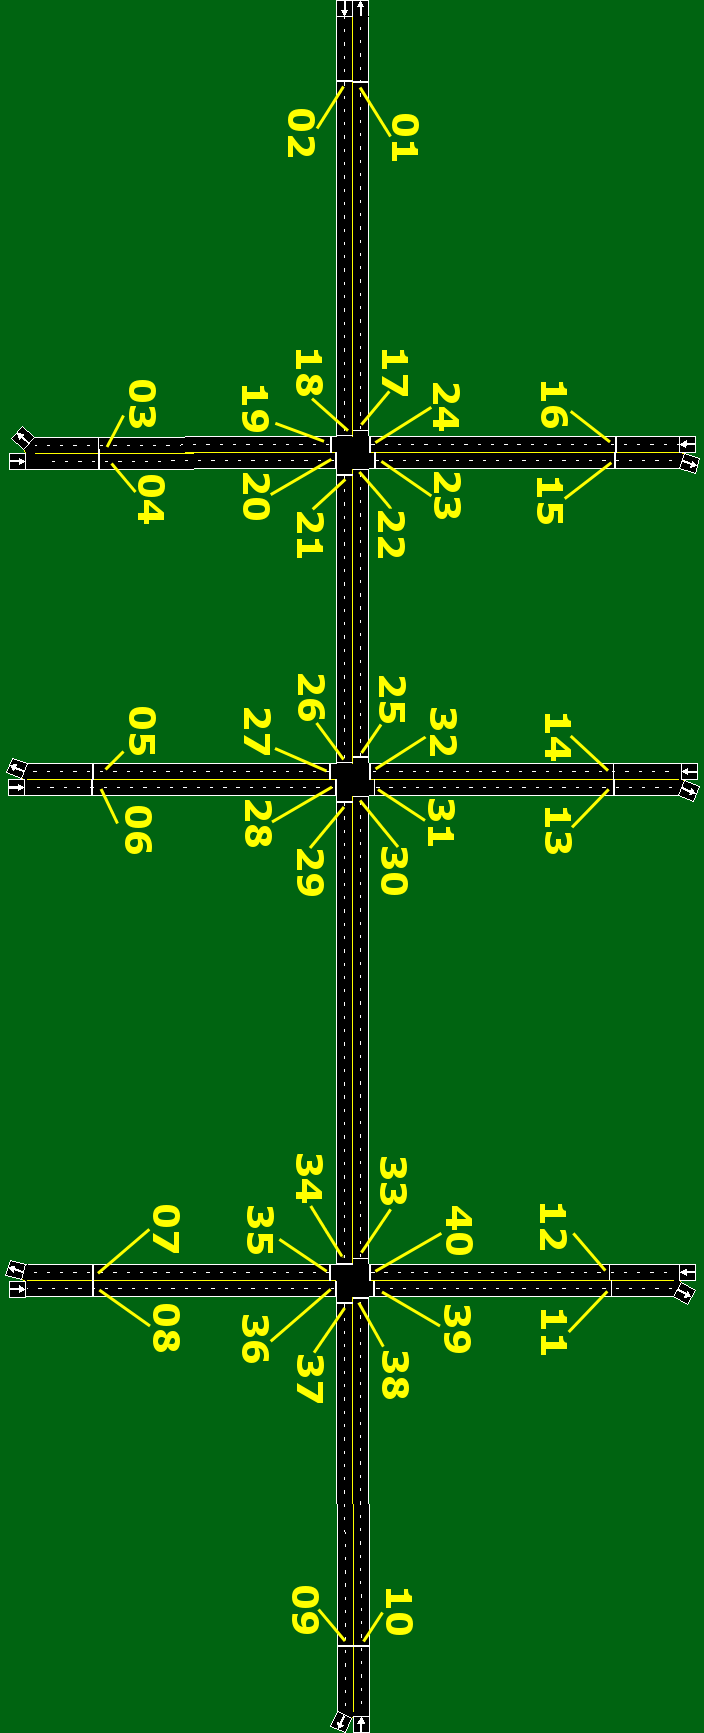
\includegraphics[width=1\columnwidth]{tsis-model-simple}
\caption[Rete stradale del dataset $1$]{File \acs{TNO} rappresentante la rete stradale da cui viene generato il dataset $1$.}
\label{fig:tsis-corsim-arch}
\end{sidewaysfigure}

\subsection{Risultati}
\omissis{}

\section{Dataset \texorpdfstring{$2$}{2}}
\omissis{}

\subsection{Modello TSIS}
\omissis{}

\subsection{Risultati}
\omissis{}
